\documentclass[10pt,border=3pt]{standalone}
\usepackage{amsmath}
\usepackage{tikz-feynman}
\tikzfeynmanset{compat=1.1.0}
\begin{document}
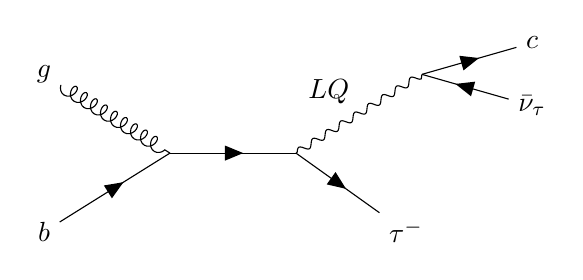
\begin{tikzpicture}
\begin{feynman}
    \vertex (g)   at (0,2.0) {$g$};
    \vertex (b)   at (0,0) {$b$};
    \vertex (v0)  at (1.6,1.0);
    \vertex (v1)  at (3.2,1.0);
    \vertex (v2)  at (4.8,2.0);
    \vertex (tau) at (4.6,0) {$\tau^-$};
    \vertex (c)   at (6.2,2.4) {$c$};
    \vertex (nu)  at (6.2,1.6) {$\bar{\nu}_{\tau}$};
    \diagram*{
        (b) -- [fermion] (v0) -- [fermion] (v1),
        (g) -- [gluon] (v0),
        (v1) -- [fermion] (tau),
        (v1) -- [boson, edge label={$LQ$}] (v2),
        (v2) -- [fermion] (c),
        (nu) -- [fermion] (v2),
    };
\end{feynman}
\end{tikzpicture}
\end{document}
